\chapter{Casi d'uso e workflow}

\section{Casi d'uso}

Nel seguente paragrafo verranno descritti i casi d'uso che l'applicazione supporta.

\subsection{Registrazione e login di un utente}

\textit{Deve essere possibile registrare un nuovo utente nel sistema e permettergli di autenticarsi.} \\

\noindent
Vi sono due tipologie di utenti, quelli interni all'ateneo (professori e studenti) e quelli esterni (aziende). Gli utenti interni devono effettuare l'accesso con il proprio account istituzionale utilizzando Google come provider federato, mentre le aziende possono inserire un'email qualunque. 

Una volta che un membro dell'ateneo esegue l'accesso mediante Google, viene reindirizzato indietro al sistema, che verifica l'email utilizzata nella fase di accesso a Google: se termina con \textit{@stud.unive} rappresenta un utente con il ruolo di studente, mentre se termina con\textit{@unive.it} rappresenta il un utente con il ruolo di professore. Una volta determinato il ruolo, il sistema verifica l'esistenza di un utente nella relativa \textit{collection} del database e in caso negativo lo crea, registrando un nuovo utente. A questo punto l'utente (professore o studente) è autenticato e viene indirizzato nella parte del portale protetta.

Per quanto riguarda un utente con il ruolo di azienda, invece, la procedura di \textit{login} e registrazione è divisa in pagine diverse. Nella pagina di registrazione l'utente deve indicare i dati della propria azienda, un'indirizzo email e una password, dopodiché verrà creato sia una nuova azienda che un nuovo utente, associando l'utente come amministratore della nuova azienda. Nella procedura di login invece, l'utente dovrà inserire l'email e la password utilizzate in fase di registrazione.

\begin{figure}[H] 
	\centering    
	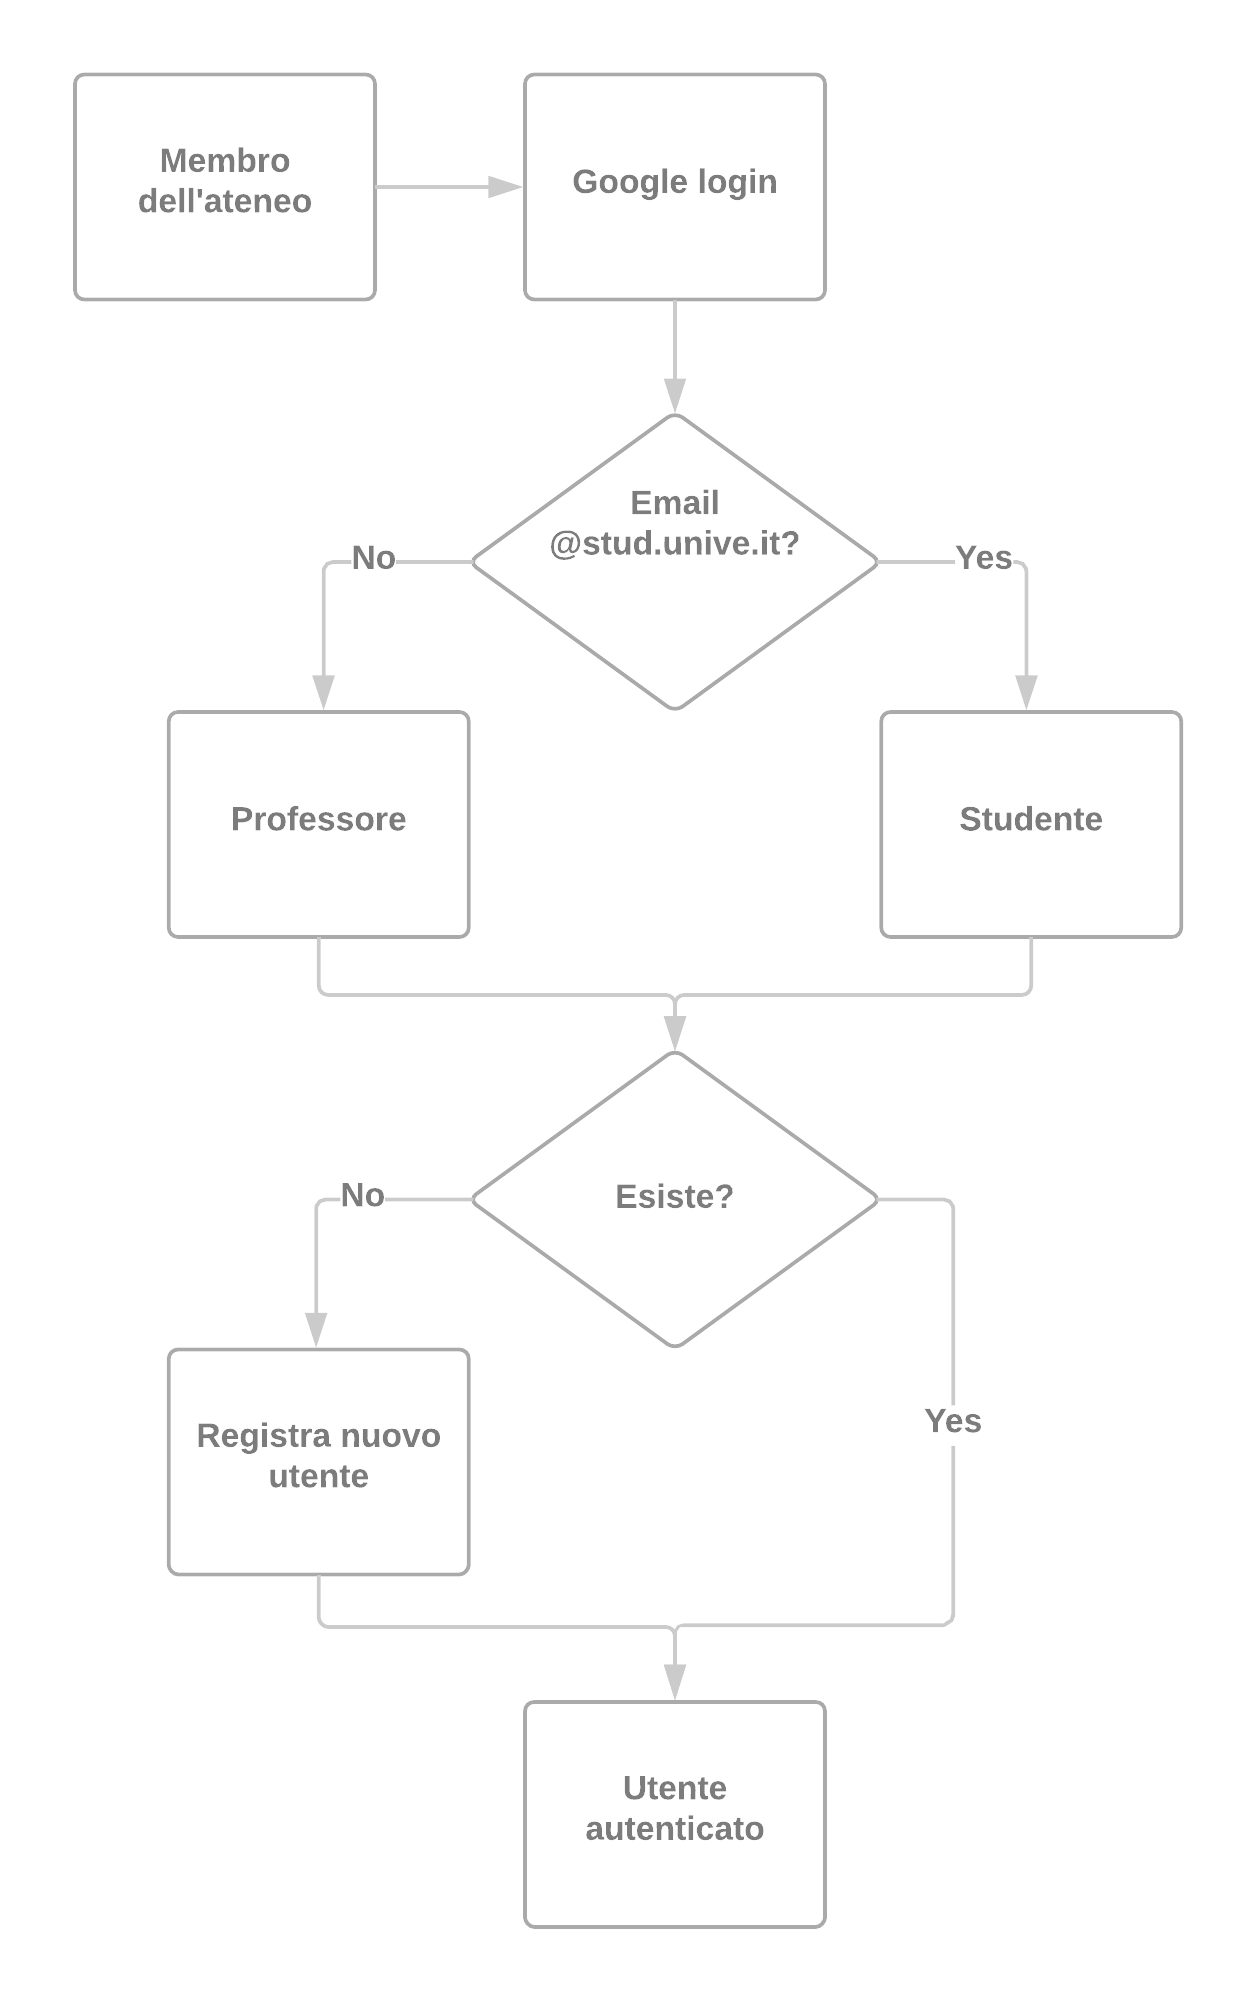
\includegraphics[width=0.4\textwidth]{Chapter2/Figs/univelogin}
	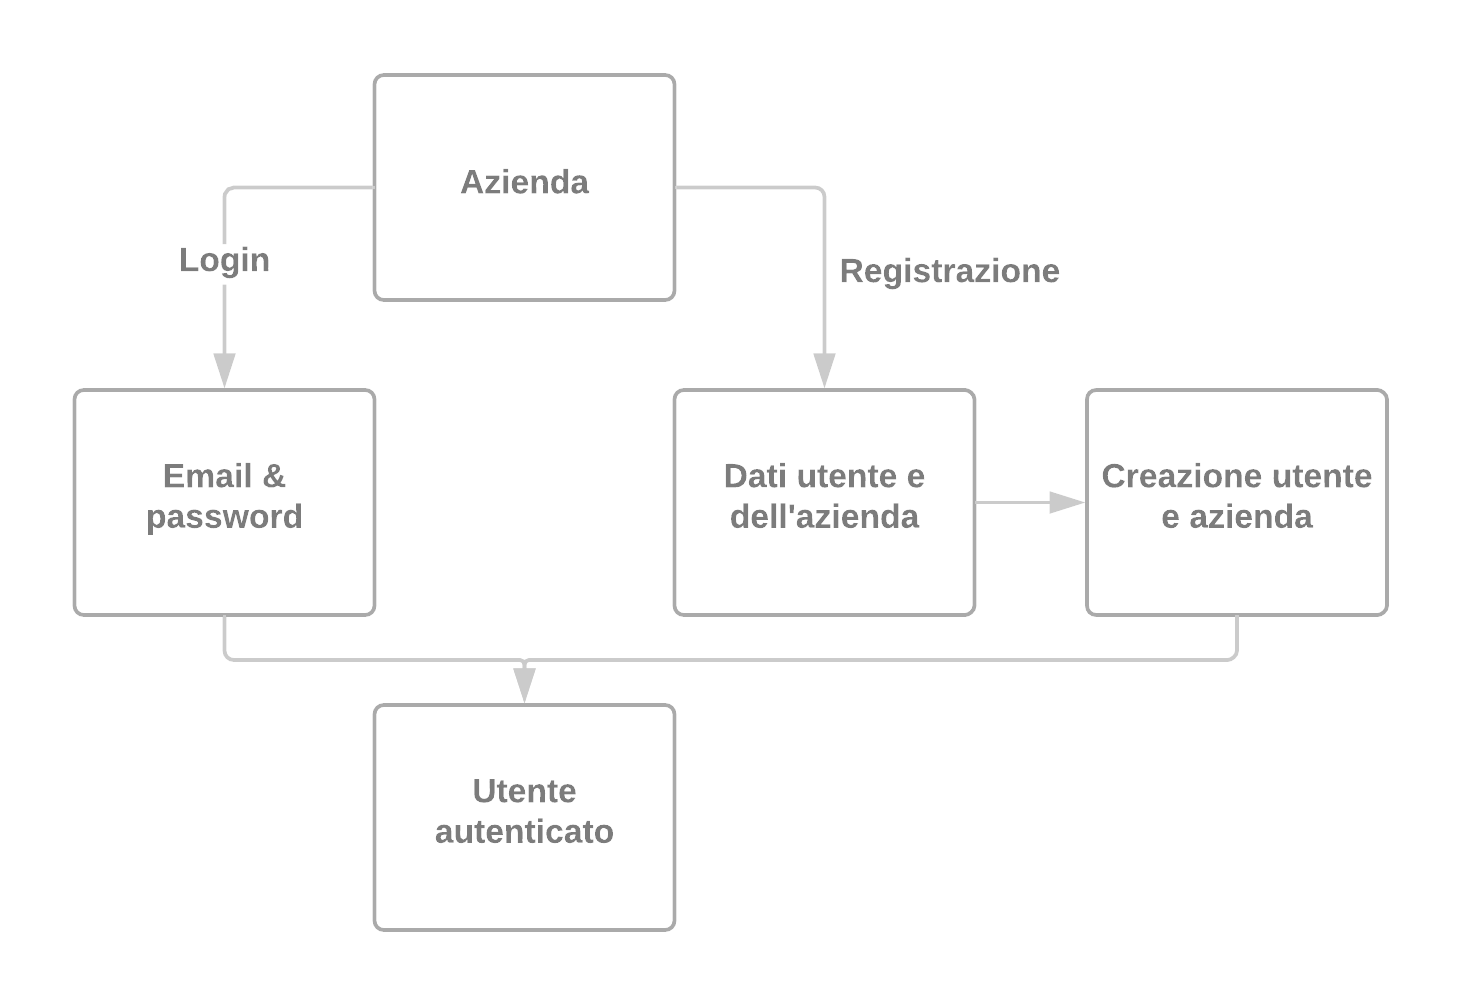
\includegraphics[width=0.5\textwidth]{Chapter2/Figs/companylogin}
	\caption[Flusso di login e registrazione di un utente]{Flusso di login e registrazione di un utente}
	\label{fig:univelogin}
\end{figure}

\subsection{Creazione di un tirocinio}

Tirocinio
\subsection{Modifica di un tirocinio}
And some more \dots

\subsection{Approvazione di un tirocinio}
And some more \dots

\subsection{Candidatura ad un tirocinio}
And some more \dots

\subsection{Approvazione candidatura (professore)}
And some more \dots

\subsection{Approvazione candidatura (azienda)}
And some more \dots

\subsection{Avvio di un tirocinio}
And some more \dots

\subsection{Compilazione foglio presenze}
And some more \dots

\subsection{Generazione documentazione}
And some more \dots